\documentclass[12pt,ngerman]{scrartcl}

\usepackage[utf8]{inputenc}
\usepackage[T1]{fontenc}
\usepackage{babel}
\usepackage{tikz}

% Sucht nach minimaltikz.pdf im Netz

\begin{document}

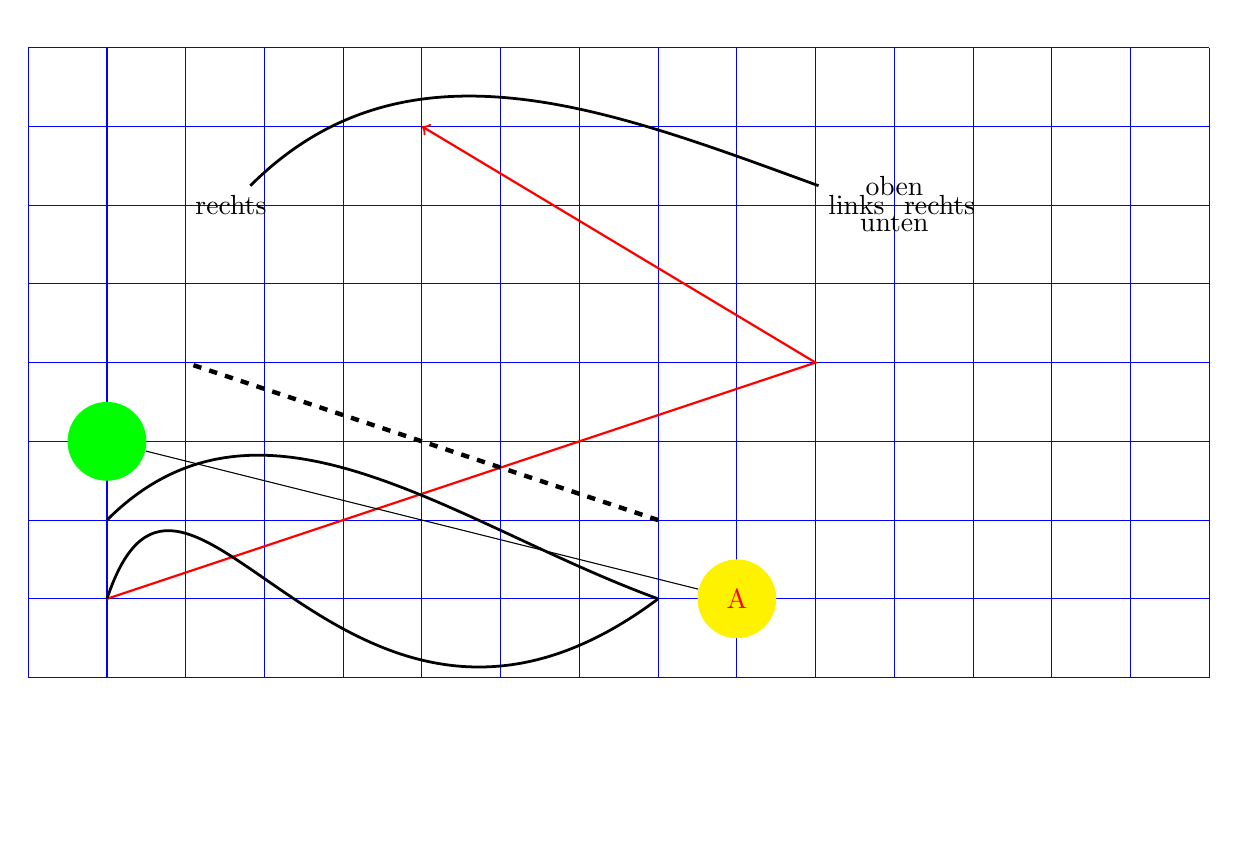
\begin{tikzpicture}
[punkt/.style={circle, minimum size = 1cm,red,fill=yellow},
punkta/.style={punkt,fill=green},
]
\draw[help lines,blue,thin] (0,0) grid (15,8);
\draw[thick,red,->] (1,1) -- (10,4) -- (5,7);
\draw[dashed, ultra thick] (8,2) -- (2,4);

\draw[line width=1pt] (1,1) .. controls (2,4) and (4,-2) .. (8,1);
\draw[line width=1pt] (1,2) to [out=45, in=160] (8,1);

\node[punkt] (A) at (9,1){A};
\node[punkta] (B) at (1,3){};
\draw (A) -- (B);

\node (C) [below] at (11,6) {unten};
\node (D) [above] at (11,6) {oben};
\node (E) [left] at (11,6) {links};
\node (F) [right] at (11,6) {rechts};

\node (G) [right] at (2,6) {rechts};

\draw[line width=1pt] (G) to [out=45, in=160] (E.north west);
\end{tikzpicture}

\end{document}


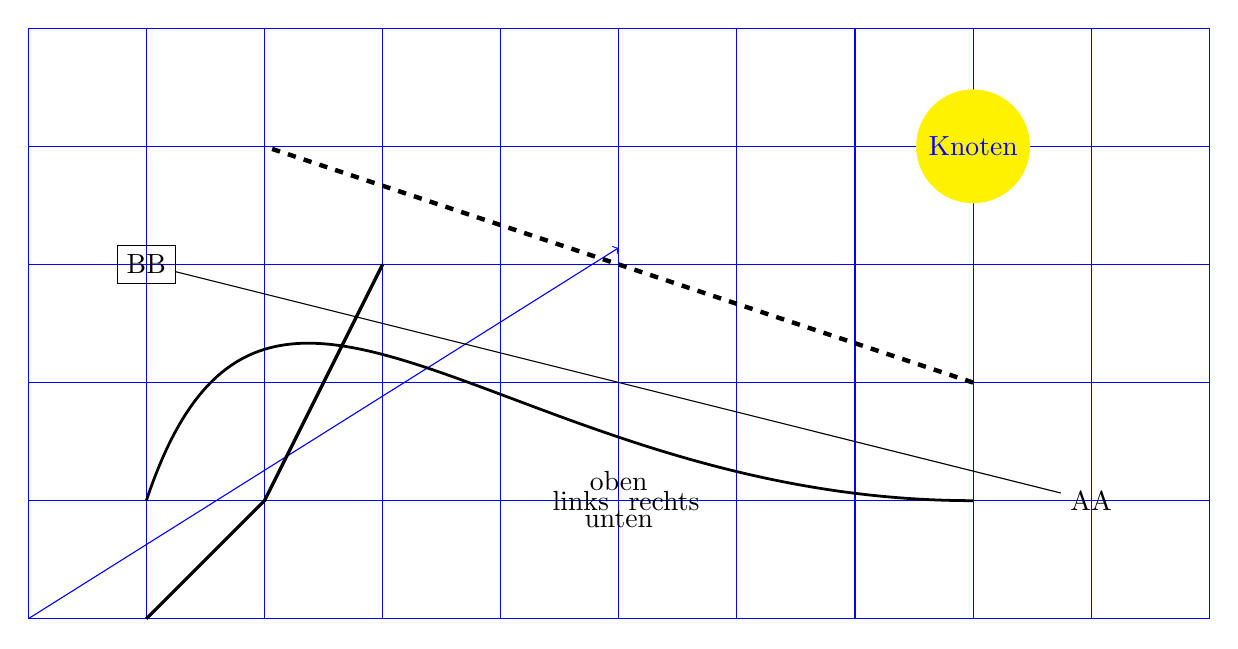
\begin{tikzpicture}[scale=1.5,
    punkt/.style={circle, minimum size = 1cm,blue,fill=yellow},
]

\draw[help lines,blue,thin] (0,0) grid (10,5);

\draw [->,thin,blue]  (0,0) -- (5,3.1415927);

\draw [very thick] (1,0) -- (2,1) -- (3,3);

\draw [dashed, ultra thick] (8,2) -- (2,4);

\node [punkt] at (8,4){Knoten};

\node [below] at (5,1) {unten};
\node [above] at (5,1) {oben};
\node [left] at (5,1) {links};
\node [right] at (5,1) {rechts};

\node (A) at (9,1){AA};
\node [draw] (B) at (1,3){BB};
\draw (A) -- (B);

\draw[line width=1pt] (1,1) .. controls (2,4) and (4,1) .. (8,1);


\end{tikzpicture}



\draw [->,very thick] (0,0) -- (5,0);
\draw [->,very thick] (0,0) -- (0,5);
\draw [very thick] (0,0) -- (1,2) -- (3,3);
\draw [dashed, ultra thick] (5,5) -- (2,2);

\node  [punkt] at (7,3){Knoten};

\node [below] at (4,2) {below};
\node [above] at (4,2) {above};
\node [left] at (4,2) {left};
\node [right] at (4,2) {right};

\node (A) at (9,1){A};
\node[draw] (B) at (8,4){B};
\draw (A) -- (B);


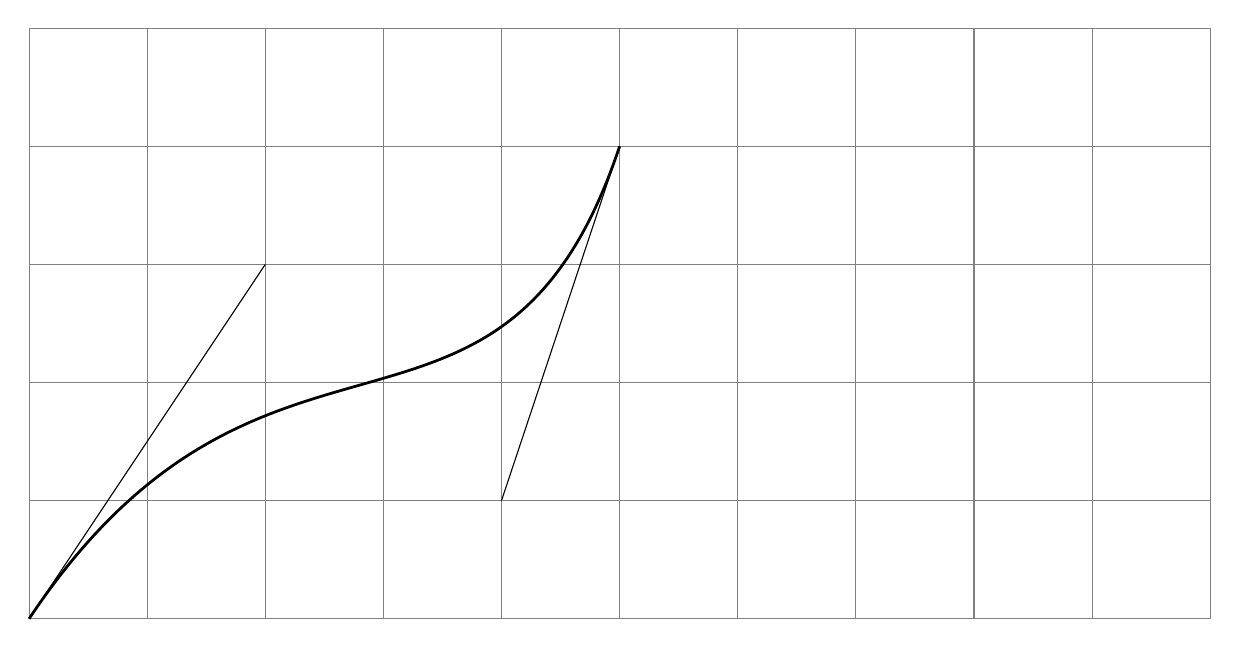
\begin{tikzpicture}[scale=1.5]
\draw[help lines,gray,thin] (0,0) grid (10,5);
\draw[line width=1pt] (0,0) .. controls (2,3) and (4,1) .. (5,4); % cubic bezier curve

\draw (0,0) -- (2,3); % (0,0) to 2. point
\draw (5,4) -- (4,1); % (1,1) to 3. point
\end{tikzpicture}